\documentclass{article}

\usepackage[margin=1in]{geometry}
\usepackage{amsmath,amsthm,amssymb}
\usepackage{bbm,enumerate,mathtools,multicol}
\usepackage[shortlabels]{enumitem}
\usepackage[hidelinks]{hyperref}
\usepackage{tikz}
\usetikzlibrary{matrix, arrows}

\newenvironment{problem}[2][Problem]{\begin{trivlist}
\item[\hskip \labelsep {\bfseries #1}\hskip \labelsep {\bfseries #2.}]}{\end{trivlist}}
\newenvironment{solution}[1][Solution.]{\begin{trivlist}
\item[\hskip \labelsep {\bfseries #1}]}{\end{trivlist}}
\newenvironment{problempart}[1]{\begin{trivlist}\item[\textbf{Part #1.}]}{\end{trivlist}}

\begin{document}

\title{Topology: Midterm corrections}
\author{Peter Kagey}

\maketitle

% -----------------------------------------------------
% First problem
% -----------------------------------------------------
\begin{problem}{1} \text{} \\
  Let $X$ be a subspace of the punctured plane $\mathbb R^2 - \{ 0 \}$ such that
  the homomorphism $\pi_1(X; x_0) \rightarrow \pi_1(\mathbb R^2 - \{ 0 \}; x_0)$
  induced by the inclusion map is
  nontrivial. Show that $X$ has a nonempty intersection with every half-line
  $L_{(a, b)} = \{ (\lambda a, \lambda b) \in \mathbb R^2; \lambda > 0\}$ issued
  from the origin (with $(a, b) \neq (0, 0)$).
\end{problem}

\begin{proof} \text{} \\
  Firstly, $\mathbb R^2 - L_{(a,b)}$ is star shaped with center $(-a, -b)$,
  so its fundamental group is trivial: \[
    \pi_1(\mathbb R^2 - L_{(a,b)}; x_0) = \mathbf{1}.
  \]
  Assume that $X$ does not include $L$. Then consider the inclusion maps and the corresponding induced homomorphisms
  \begin{alignat*}{5}
    &X
    &&\xrightarrow{i_1} &&\mathbb R^2 - L_{(a,b)}
    &&\xrightarrow{i_2} &&\mathbb R^2 - \{ 0 \} \\
    \pi_1(&X; x_0)
    &&\xrightarrow{i_{1*}} \pi_1(&&\mathbb R^2 - L_{(a,b)}; x_0)
    &&\xrightarrow{i_{2*}} \pi_1(&&\mathbb R^2 - \{ 0 \}; x_0)\\
    \pi_1(&X; x_0)
    &&\xrightarrow{i_{1*}} &&\mathbb \mathbf{1}
    &&\xrightarrow{i_{2*}} &&\mathbb Z
  \end{alignat*}
  Since $i_{2*}\colon \mathbf{1}\rightarrow\mathbb Z$ is trivial, the
  homomorphism induced from the inclusion map
  \[
    i_{2*} \circ i_{1*} = (i_{2} \circ i_{1})_*\colon\pi_1(\mathbb R^2 - L_{(a,b)}; x_0) \rightarrow\pi_1(\mathbb R^2 - \{ 0 \}; x_0)
  \]
  must also be trivial.

  This is a contradiction of the hypothesis, so $X$ must intersect $L$.
\end{proof}
\pagebreak
% -----------------------------------------------------
% Second problem
% -----------------------------------------------------
\begin{problem}{2} \text{} \\
  Let $X$ be a path connected space whose fundamental group $\pi_1(X; x_0)$ is
  isomorphic to $\mathbb Z \times \mathbb Z_2 \times \mathbb Z_3 \times \mathbb Z_5$.
  Show that the change of basepoint isomorphism
  $T_\gamma\colon\pi_1(X;y_0) \rightarrow \pi_1(X;x_0)$ defined by
  $T_\gamma([\alpha]) = [\gamma * \alpha * \overline\gamma]$ for some path from
  $x_0$ to $y_0$ depends only on the endpoints $x_0$ and $y_0$ and does not
  depend on the path $\gamma$.
\end{problem}

\begin{proof} \text{} \\
  We will exploit the fact that $\pi_1(X; x_0)$ is abelian.
  Consider two different paths, $\gamma_1$ and $\gamma_2$, and an element of
  $[\alpha] \in \pi_1(X; y_0)$. It is suffient to show that
  $T_{\gamma_1}([\alpha]) = T_{\gamma_2}([\alpha]) \in \pi_1(X; x_0)$, which is
  to say, we want to show that \[
    [\gamma_1 * \alpha * \overline\gamma_1] \cdot [\gamma_2 * \alpha * \overline\gamma_2]^{-1}
    = \operatorname{id}_{\pi_1(X; x_0)}.
  \]
  Notice that $\overline\gamma_1 * \gamma_2$ is a path from $y_0$ to $x_0$
  concatenated with a path from $x_0$ to $y_0$, and thus
  $[\overline\gamma_1 * \gamma_2] \in \pi_1(X; y_0)$.
  Since $\pi_1(X; y_0) \cong \mathbb Z \times \mathbb Z_2 \times \mathbb Z_3 \times \mathbb Z_5$ is abelian, the product can be rearranged as follows:
  \begin{align*}
    [\alpha * \overline\gamma_1 * \gamma_2 * \overline\alpha]
    &= [\alpha] \cdot [\overline\gamma_1 * \gamma_2] \cdot [\overline\alpha] \\
    &= [\alpha] \cdot [\overline\alpha] \cdot [\overline\gamma_1 * \gamma_2] \\
    &= [\alpha * \overline\alpha] \cdot [\overline\gamma_1 * \gamma_2] \\
    &= [\overline\gamma_1 * \gamma_2]
  \end{align*} so in particular,
  $\alpha * \overline\gamma_1 * \gamma_2 * \overline\alpha \cong \overline\gamma_1 * \gamma_2$.
  Since $[\gamma * \alpha * \overline\gamma]^{-1} = [\gamma * \overline\alpha * \overline\gamma]$
  by tracing the path backward, this is equivalent to \begin{align*}
    [\gamma_1 * \alpha * \overline\gamma_1] \cdot [\gamma_2 * \alpha * \overline\gamma_2]^{-1}
    &= [\gamma_1 * \alpha * \overline\gamma_1] \cdot [\gamma_2 * \overline\alpha * \overline\gamma_2]\\
    &= [\gamma_1 * \underbrace{\alpha * \overline\gamma_1 * \gamma_2 * \overline\alpha}_{\simeq \overline\gamma_1 * \gamma_2} * \overline\gamma_2] \\
    &= [\gamma_1 * \overline\gamma_1 * \gamma_2 * \overline\gamma_2] \\
    &= [c_{x_0}]
  \end{align*}
  Therefore $[\gamma_1 * \alpha * \overline\gamma_1] \cdot [\gamma_2 * \alpha * \overline\gamma_2]^{-1} = [c_{x_0}]$.
  Thus for every $[\alpha] \in \pi_1(X;y_0)$, $T_{\gamma_1}([\alpha]) = T_{\gamma_2}([\alpha])$,
  the change of basepoint isomorphism does not depend on the path when the fundamental group is abelian.
\end{proof}
\pagebreak
% -----------------------------------------------------
% Third problem
% -----------------------------------------------------
\begin{problem}{3} \text{} \\
  For positive integers $m, n \geq 1$, let
  $i_n\colon\mathbb Z_2 \rightarrow Z_{2n} = \langle a; a^{2n} = 1 \rangle$
  denote the homomorphism that sends the nontrivial element of
  $\mathbb Z_2$ to $a^n$, and let
  $\mathbb Z_{2m} *_{\mathbb Z_2} \mathbb Z_{2n}$ be the amalgamated free
  product defined by the homomorphisms $i_m$ and $i_n$.
  \begin{enumerate}[a.]
    \item Show that $\mathbb Z_2 *_{\mathbb Z_2} \mathbb Z_{2n}$ is abelian.
    \item Construct a surjective group homomorphism \[
      \varphi\colon\mathbb Z_{2m} *_{\mathbb Z_2} \mathbb Z_{2n}
      \rightarrow \mathbb Z_m * \mathbb Z_n.
    \]
    \item Show that $\mathbb Z_{2m} *_{\mathbb Z_2} \mathbb Z_{2n}$ is not
    abelian when $m, n \geq 2$.
  \end{enumerate}
\end{problem}

\begin{proof} \text{} \\
  \begin{enumerate}[a.]
    \item Name the amalgamated product $G$ and write it as
    $G = \langle a; a^2 = 1\rangle *_{\mathbb Z_2} \langle b; b^{2n} = 1\rangle$.
    By the maps $1 \xmapsto{i_1} a$ and $1 \xmapsto{i_n} b^n$, we can write
    $G$ via the group presentation \[
      G = \langle a, b; a = b^n, a^2 = b^{2n} = 1 \rangle \cong \mathbb Z_{2n},
    \]
    which is abelian.
    \item Name the amalgamated product $G$ and write it as
    $G = \langle a; a^{2m} = 1\rangle *_{\mathbb Z_2} \langle b; b^{2n} = 1\rangle$.
    Similarly, by the maps
    $1 \xmapsto{i_m} a^m$ and $1 \xmapsto{i_n} b^n$, we can write $G$ via the
    group presentation \[
      G = \langle a, b; a^mb^{-n} = a^{2m} = b^{2n} = 1 \rangle.
    \]
    By the universal property of free products, given the homomorphisms \begin{align*}
      j_A \colon \langle a \rangle \rightarrow
      \langle c; c^{m} = 1 \rangle
      * \langle d; d^{n} = 1 \rangle
      \text{ which sends } a \mapsto d
      \\
      j_B \colon \langle b \rangle \rightarrow
      \langle c; c^{m} = 1 \rangle
      * \langle d; d^{n} = 1 \rangle
      \text{ which sends } b \mapsto c
    \end{align*}
    there exists a map \[
      \varphi\colon \langle a \rangle * \langle b \rangle
      \rightarrow \langle c; c^{m} = 1 \rangle * \langle d; d^{n} = 1 \rangle
    \] which sends $a \mapsto c$ and $b \mapsto d$ is a homomorphism.
    In particular, the relations of $G$ are in the kernel of this map: \begin{align*}
      \varphi(a^m b^{-n})
        &= \varphi(a)^m\varphi(b^{-1})^n
        = \underbrace{c^m}_{1 \in \mathbb Z_m} \underbrace{(d^{-1})^n}_{1 \in \mathbb Z_n}
        = 1
      \\
      \varphi(a^{2m})
        &= \varphi(a^2)^m
        = (c^2)^m
        = 1 \in \mathbb Z_m
      \\
      \varphi(b^{2n})
        &= \varphi(b^2)^n
        = (d^2)^n
        = 1 \in \mathbb Z_n.
    \end{align*}
    Therefore we can write our desired homomorphism as
    $\varphi'\colon G \rightarrow \langle c; c^{m} = 1 \rangle * \langle d; d^{n} = 1 \rangle$
    which sends $a\xmapsto{\varphi'}c$ and $b\xmapsto{\varphi'}d$.
    \\
    This map is surjective because we can write any element \[
      c^{i_1}d^{i_2}c^{i_3}d^{i_4}\hdots c^{i_{n-1}}d^{i_n} \in
      \langle c; c^m = 1 \rangle * \langle d; d^n = 1 \rangle
    \]
    as $\varphi(a^{i_1}\cdot b^{i_2}\cdot a^{i_3}\cdot b^{i_4}\hdots \cdot a^{i_{n-1}}\cdot b^{i_n})$.

    \item The surjective homomorphism $\varphi$, which is described above, maps
    $\mathbb Z_{2m} *_{\mathbb Z_2} \mathbb Z_{2n}$ onto the free
    group on two letters, which is not commutative. Since homomorphisms preserve
    commutivity, $\mathbb Z_{2m} *_{\mathbb Z_2} \mathbb Z_{2n}$ is not abelian.
  \end{enumerate}
\end{proof}
\pagebreak
% -----------------------------------------------------
% Third problem
% -----------------------------------------------------
\begin{problem}{4} \text{} \\
  Let $X$ be the quotient space of the annulus $S^1 \times [0, 1]$ by the
  equivalence relation $\sim$ which identifies each point $(z, 0)$ to $(-z, 0)$ and
  each point $(z, 1)$ to $(-z, 1)$. Compute the fundamental group of $X$.
\end{problem}
\begin{proof}
  We will use van Kampen with the a cut along $S^1 \times \{ 1/2 \} \simeq S^1$:
  \\
  \begin{figure}[h]
    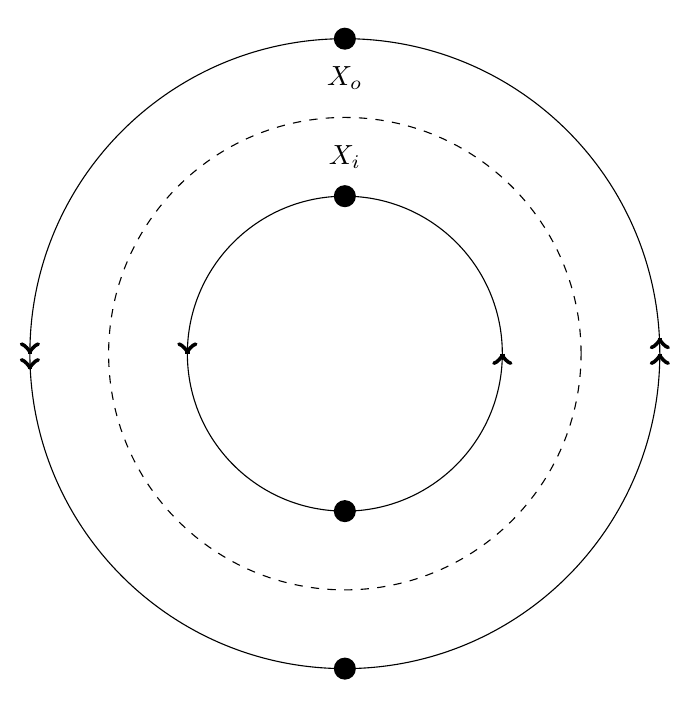
\begin{tikzpicture}
      \draw (0,0) circle (4);
      \node () at (0, 3.5) {$X_o$};
      \fill (0,4) circle (0.14);
      \fill (0,-4) circle (0.14);
      \draw[ultra thick, ->] (4,0)--(4,0.001);
      \draw[ultra thick, ->] (4,0.2)--(4,0.201);
      \draw[ultra thick, ->] (-4,0)--(-4,-0.001);
      \draw[ultra thick, ->] (-4,-0.2)--(-4,-0.201);

      \draw (0,0) circle (2);
      \node () at (0, 2.5) {$X_i$};
      \fill (0,2) circle (0.14);
      \fill (0,-2) circle (0.14);
      \draw[ultra thick, ->] (2,0)--(2,0.001);
      \draw[ultra thick, ->] (-2,0)--(-2,-0.001);

      \draw[dashed] (0,0) circle (3);
    \end{tikzpicture}
  \end{figure}\\
  Let $X_o$ be the outer part of the annulus with the outer boundary identified,
  and  let $X_i$ be the inner part of the annulus with the inner boundary
  identified. Since both $X_o$ and $X_i$ have a deformation retract to their
  respective boundaries,
  $\pi_1(X_o; x_0) \cong \pi_1(X_i; x_0) \cong \mathbb Z$, where $x_0$ is a
  point on $S^1 \times [0, 1]$.
  Then the fundamental group is given by the amalgamated product \begin{align*}
    \pi_1(X; x_0) &= \pi_1(X_o; x_0) *_{\pi_1(S_1; x_0)} \pi_1(X_i; x_0) \\
    &\cong \mathbb Z *_{\mathbb Z} \mathbb Z \\
    &\cong \langle a \rangle *_{\langle b \rangle} \langle c \rangle
  \end{align*}
  with maps \begin{alignat*}{2}
    i_o\colon \langle b \rangle &\rightarrow \langle a \rangle
    \hspace{1cm}\text{sending}\hspace{1cm}
    b &&\mapsto a^2
    \\
    i_i\colon \langle b \rangle &\rightarrow \langle c \rangle
    \hspace{1cm}\text{sending}\hspace{1cm}
    b &&\mapsto c^2.
  \end{alignat*}
  Since a loop around the interior of the annulus maps to a loop twice around
  the boundary under the deformation retract.
  \\
  Therefore, the resulting amalgamated product is \[
    \pi_1(X; x_0) = \langle a, c; a^2 = c^2 \rangle.
  \]
  % The procedure I will use is to use the van Kampen theorem to identify the
  % outer boundary and get $X'$ (which I believe is the Mobius strip) and then use
  % the van Kampen theorem again to identify the inner boundary. We can do this
  % because there is a deformation retract from the annulus to its
  % outer boundary, and a neighborhood deformation retract from the circle to the
  % circle with antipodal points identified.
  % In particular \begin{align*}
  %   \pi_1(X'; x_0) &= \pi_1(S^1 \times [0, 1]; x_0) *_{\pi_1(S^1; x_0)} \pi_1(S^1; x_0) \\
  %   &= \mathbb Z *_{\mathbb Z} \mathbb Z \\
  %   &= \langle a \rangle *_{\mathbb Z} \langle c \rangle
  % \end{align*}
  % with maps \begin{alignat*}{2}
  %   i_A\colon \mathbb Z &\rightarrow \langle a \rangle &&\text{ by } 1 \mapsto a \text{ and }\\
  %   i_C\colon \mathbb Z &\rightarrow \langle c \rangle &&\text{ by } 1 \mapsto c^2
  % \end{alignat*}
  % where $a$ counts the number of loops around the annulus and $b$ counts loops
  % around the outer boundary. The second map is a consequence of the fact that
  % one loop around the annulus is homeomorphic to two loops around the outer
  % boundary.
  % Thus the group representation for the fundamental group of the annulus with the
  % antipodal points of the outer boundary identified is
  % \[\pi_1(X'; x_0) = \langle a, c ; a = c^2 \rangle \cong \mathbb Z.\]
  % Repeating the process with the inner annulus gives the fundamental group of
  % $X$, \begin{align*}
  %   \pi_1(X'; x_0) &= \pi_1(X'; x_0) *_{\pi_1(S^1; x_0)} \pi_1(S^1; x_0) \\
  %                  &= \langle a, c ; a = c^2 \rangle *_{\mathbb Z} \langle b; \rangle
  % \end{align*}
  % with maps \begin{alignat*}{2}
  %   i_A\colon \mathbb Z &\rightarrow \langle a \rangle &&\text{ by } 1 \mapsto a \text{ and }\\
  %   i_B\colon \mathbb Z &\rightarrow \langle c \rangle &&\text{ by } 1 \mapsto b^2.
  % \end{alignat*}
  % Therefore the group representation for the fundamental group of $X$ has group
  % representation \[
  %   \pi_1(X; x_0) = \langle a, b, c ; b^2 = a = c^2 \rangle \cong \langle b, c ; b^2 = c^2 \rangle.
  % \]
\end{proof}
\end{document}
